\chapter{Interlude: eighteen examples of affine schemes}
\label{ch:spec_examples}
To cement in the previous two chapters,
we now give an enormous list of examples.
Each example gets its own section,
rather than having page-long orange boxes.

One common theme you will find as you wade through
the examples is that your geometric intuition may
be better than your algebraic one.
For example, while studying $k[x,y] / (xy)$ you will say
``geometrically, I expect so-and-so to look like other thing'',
but when you write down the algebraic statements
you find two expressions that are don't look equal to you.
However, if you then do some calculation you will
find that they were isomorphic after all.
So in that sense, in this chapter you will learn to begin drawing
pictures of algebraic statements --- which is great!

As another example, all the lemmas about
prime ideals from our study of localizations
will begin to now take concrete forms:
you will see many examples that
\begin{itemize}
	\ii $\Spec A/I$ looks like $\VV(I)$ of $\Spec A$,
	\ii $\Spec A[1/f]$ looks like $D(f)$ of $\Spec A$,
	\ii $\Spec A_\kp$ looks like $\OO_{\Spec A, \kp}$ of $\Spec A$.
\end{itemize}

In everything that follows, $k$ is any field.
We will also use the following color connotations:
\begin{itemize}
	\ii The closed points of the scheme are drawn in blue.
	\ii Non-closed points are drawn in red,
	with their ``trails'' dotted red.
	\ii Stalks are drawn in green, when they appear.
\end{itemize}


\section{Example: $\Spec k$, a single point}
This one is easy: for any field $k$,
$X = \Spec k$ has a single point,
corresponding to the only proper ideal $(0)$.
There is only way to put a topology on it.

As for the sheaf,
\[ \OO_X(X) = \OO_{X,(0)} = k. \]
So the space is remembering what field it wants to be over.
If we are complex analysists,
the set of functions on a single point is $\CC$;
if we are number theoerists,
maybe the set of functions on a single point is $\QQ$.

%%fakechapter One-dimensional
\section{$\Spec \CC[x]$, a one-dimensional line}
The scheme $X = \Spec \CC[x]$ is our beloved one-dimensional line.
It consists of two types of points:
\begin{itemize}
	\ii The closed points $(x-a)$, corresponding to each
	complex number $a \in \CC$, and
	\ii The \emph{generic} point $(0)$.
\end{itemize}
As for the Zariski topology, every open set contains $(0)$,
which captures the idea it is close to everywhere:
no matter where you stand, you can still here the buzzing of the fly!
True to the irreducibility of this space,
the open sets are huge:
the proper \emph{closed sets} consist of finitely many closed points.

Here is a picture:
for lack of better place to put it,
the point $(0)$ is floating around just above the line in red.
\begin{center}
	\begin{asy}
		size(8cm);
		pair A = (-8,0); pair B = (8,0);
		draw(A--B, blue, Arrows);
		dot("$(x)$", (0,0), dir(-90), blue);
		dot("$(x-3)$", (3,0), dir(-90), blue);
		dot("$(x+i)$", (-4,0), dir(-90), blue);
		dot("$(0)$", (0,1), dir(90), red);
		draw( (-6,0)..(-3,0.5)..(-1,1)--(1,1)--(3,0.5)--(6,0), dotted+red );
		label("$\operatorname{Spec} \mathbb C[x]$", A, dir(-90), blue);
	\end{asy}
\end{center}

The notion of ``value at $\kp$'' works as expected.
For example, $f = x^2+5$ is a global section of $\CC[x]$.
If we evaluate it at $\kp = x-3$,
we find $f(\kp) = f \pmod \kp = x^2+5 \pmod{x-3} = 14 \pmod{x-3}$.
Indeed, \[ \kappa(\kp) \cong \CC \]
meaning the stalks all have residue field $\CC$.
As \[ \CC[x] / \kp \cong \CC \qquad \text{by $x \mapsto 3$} \]
we see we are just plugging $x=3$.

Of course, the stalk at $(x-3)$ carries more information.
In this case it is $\CC[x]_{(x-3)}$.
Which means that if we stand near the point $(x-3)$,
rational functions are all fine as long as no $x-3$
appears in the denominator.
So, $\frac{x^2+8}{(x-1)(x-5)}$ is a fine example of a germ near $x=3$.

Things get more interesting if we
consider the generic point $\eta = (0)$.

What is the stalk $\OO_{X, \eta}$?
Well, it should be $\CC[x]_{(0)} = \CC(x)$,
which is the again the set of \emph{rational} functions.
And that's what you expect.
For example, $\frac{x^2+8}{(x-1)(x-5)}$
certainly describes a rational function on ``most'' complex numbers.

What happens if we evaluate the global section
$f = x^2+5$ at $\eta$?
Well, we just get $f(\eta) = x^2+5$ ---
taking modulo $0$ doesn't do much.
Fitting, it means that if you want to be able to evaluate
a polynomial $f$ at a general complex number,
you actually just need the whole polynomial
(or rational function).
We can think of this in terms of the residue field being $\CC(x)$:
\[ \kappa( (0) ) = \Frac \left( \CC[x] / (0) \right)
	\cong \Frac \CC[x] = \CC(x). \]

\section{$\Spec \RR[x]$, a one-dimensional line
with complex conjugates glued (no fear nullstellensatz)}

Despite appearances, this actually
looks almost exactly like $\Spec \CC[x]$,
even more than you expect.
The main thing to keep in mind is that now $(x^2+1)$
is a point, which you can loosely think of as $\pm i$.
So it almost didn't matter that $\RR$ is not algebraically closed;
the $\CC$ is showing through anyways.
But this time, because we only consider
real coefficient polynomials,
we do not distinguish between ``conjugate'' $+i$ and $-i$.
Put another way, we have folded $a+bi$ and $a-bi$ into a single point:
$(x+i)$ and $(x-i)$ merge to form $x^2+1$.

To be explicit, there are three types of points:
\begin{itemize}
	\ii $(x-a)$ for each real number $a$
	\ii $(x^2-ax+b)$ if $a^2 < 4b$, and
	\ii the generic point $(0)$, again.
\end{itemize}
The ideals $(x-a)$ and $(x^2-ax+b)$
are each closed points:
the quotients with $\RR[x]$ are both fields
($\RR$ and $\CC$, respectively).

We have been drawing $\Spec \CC[x]$ as a one-dimensional line,
so $\Spec \RR[x]$ will be drawn the same way.
\begin{center}
	\begin{asy}
		size(8cm);
		pair A = (-8,0); pair B = (8,0);
		draw(A--B, blue, Arrows);
		dot("$(x)$", (0,0), dir(-90), blue);
		dot("$(x-3)$", (3,0), dir(-90), blue);
		dot("$(x^2+1)$", (-4,0), dir(-90), blue);
		dot("$(0)$", (0,1), dir(90), red);
		draw( (-6,0)..(-3,0.5)..(-1,1)--(1,1)--(3,0.5)--(6,0), dotted+red );
		label("$\operatorname{Spec} \mathbb R[x]$", A, dir(-90), blue);
	\end{asy}
\end{center}

One nice thing about this is that the nullstellensatz
is less scary than it was with classical varieties.
The short version is that the function $x^2+1$
vanishes at a point of $\Spec \RR[x]$, namely $(x^2+1)$ itself!
(So in some ways we're sort of automatically working
with the algebraic closure.)

You might remember a long time ago we made a big fuss about
the weak nullstellensatz, for example in
\Cref{prob:complex_variety_nonempty}:
if $I$ was a proper ideal in $\CC[x_1, \dots, x_n]$
there was \emph{some} point $(a_1, \dots, a_n) \in \CC^n$
such that $f(a_1, \dots, a_n) = 0$ for all $f \in I$.
With schemes, it doesn't matter anymore:
if $I$ is a proper ideal of a ring $A$,
then some maximal ideal contains it,
and so $\VV(I)$ is nonempty in $\Spec A$.

We better mention that the stalks this time look different than expected.
Here are some examples:
\begin{align*}
	\kappa\left( (x^2+1) \right) &\cong \RR[x]/(x^2+1) \cong \CC \\
	\kappa \left( (x-3) \right) &\cong \RR[x] / (x-3) \cong \RR \\
	\kappa \left( (0) \right) &\cong \Frac(\RR[x] / (0)) \cong \RR(x)
\end{align*}
Notice the residue fields above the ``complex''
points are bigger: functions on them take values in $\CC$.


\section{$\Spec k[x]$, over any ground field}
In general, if $\ol k$ is the algebraic closure of $k$,
then $\Spec k[x]$ looks like $\Spec \ol k[x]$
with all the Galois conjugates glued together.
So we will almost never need ``algebraically closed''
hypotheses anymore: we're working with polynomial ideals,
so all the elements are implicitly there, anyways.

\section{$\Spec \ZZ$, a one-dimensional scheme}
The great thing about $\Spec \ZZ$ is that
it basically looks like $\Spec k[x]$, too,
being a one-dimensional scheme.
It has two types of prime ideals:
\begin{itemize}
	\ii $(p)$, for every rational prime $p$,
	\ii and the generic point $(0)$.
\end{itemize}
So the picture almost does not change.
\begin{center}
	\begin{asy}
		size(8cm);
		pair A = (-8,0); pair B = (8,0);
		draw(A--B, blue, Arrows);
		dot("$(7)$", (0,0), dir(-90), blue);
		dot("$(3)$", (3,0), dir(-90), blue);
		dot("$(19)$", (-4,0), dir(-90), blue);
		dot("$(0)$", (0,1), dir(90), red);
		draw( (-6,0)..(-3,0.5)..(-1,1)--(1,1)--(3,0.5)--(6,0), dotted+red );
		label("$\operatorname{Spec} \mathbb Z$", A, dir(-90), blue);
	\end{asy}
\end{center}
This time $\eta = (0)$ has stalk $\ZZ_{(0)} = \QQ$,
so a ``rational function'' is literally a rational number!
Thus, $\frac{20}{19}$ is a function
with a double root at $(2)$, a root at $(5)$,
and a simple pole at $(19)$.
If we evaluate it at $\kp = (7)$, we get $3 \pmod 7$.
In general, the residue fields are what you'd guess:
\[ \kappa\left( (p) \right) = \ZZ/(p) \cong \FF_p \]
for each prime $p$, and
$\kappa\left( (0) \right) \cong \QQ$.

The stalk is bigger than the residue field at the closed points:
for example
\[ \OO_{\Spec \ZZ, (3)}
	\cong \left\{ \frac mn \mid 3 \nmid n \right\} \]
consists of rational numbers with no pole at $3$.
The stalk at the generic point is $\ZZ_{(0)} \cong \Frac \ZZ = \QQ$.

%%fakechapter 0D from 1D
\section{$\Spec k[x] / (x^2-x)$, two points}
If we were working with affine varieties,
you would already know what the answer is:
$x^2-x = 0$ has solutions $x=0$ and $x=1$,
so this should be a scheme with two points.

To see this come true, we use \Cref{prop:prime_quotient}:
the points of $\Spec k[x]/(x^2-x)$
should correspond to prime ideals of $k[x]$
contained in $(x^2-x)$.
As $k[x]$ is a PID, there are only two, $(x-1)$ and $(x)$.
They are each maximal,
since their quotient with $k[x]$ is a field (namely $k$),
so as promised $\Spec k[x] / (x^2-x)$ has just two closed points.

Each point has a stalk above it isomorphic to $k$.
A section on the whole space $X$ is just a choice
of two values, one at $(x)$ and one at $(x-1)$.
\begin{center}
\begin{asy}
	size(3cm);
	draw("$k$", (-2,0)--(-2,5), dir(180), heavygreen);
	draw("$k$", (2,0)--(2,5), heavygreen);
	dot("$(x)$", (-2,0), dir(-90), blue);
	dot("$(x-1)$", (2,0), dir(-90), blue);
	label("$\operatorname{Spec} k[x]/(x^2-x)$", (0,5), 2*dir(90));
\end{asy}
\end{center}
So actually, this is a geometric way of thinking about the
ring-theoretic fact that
\[ k[x] / \left( x^2-x \right) \cong k \times k
	\quad\text{by } f \mapsto \left( f(0), f(1) \right).  \]

Also, this is the first example of a reducible space in this chapter:
in fact $X$ is even disconnected.
Accordingly there is no generic point floating around:
as the space is discrete, all points are closed.

\section{$\Spec k[x]/(x^2)$, the double point}
We can now elaborate on the ``double point'' scheme
\[ X_2 = \Spec k[x] / (x^2) \]
since it is such an important motivating example.
How it does differ from the ``one-point'' scheme
$X_1 = \Spec k[x] / (x) = \Spec k$?
Both $X_2$ and $X_1$ have exactly one point,
and so obviously the topologies are the same too.

The difference is that the stalk
(equivalently, the section, since we have only one point)
is larger:
\[ \OO_{X_2, (x)} = \OO_{X_2}(X_2)  = k[x]/(x^2). \]
So to specify a function on a double point,
you need to specify two parameters, not just one:
if we take a polynomial
\[ f = a_0 + a_1 x + \dots \in k[x] \]
then evaluating it at the double point
will remember both $a_0$ and the ``first derivative'' say.

I should mention that if you drop all the way to the residue fields,
you can't tell the difference between
the double point and the single point anymore.
For the residue field of $\Spec k[x] / (x^2)$ at $(x)$ is
\[ \Frac\left( A / (x) \right) = \Frac k = k. \]
Thus the set of \emph{values} is still just $k$
(leading to the ``nilpotent'' discussion at the end of last chapter);
but the stalk, having ``enriched'' values,
can tell the difference.

\section{$\Spec k[x]/(x^3-x^2)$, a double point and a single point}
There is no problem putting the previous two examples side by side:
the scheme $X = \Spec k[x] / (x^3-x^2)$
consists of a double point next to a single point.
Note that the stalks are different:
the one above the double point is larger.
\begin{center}
\begin{asy}
	size(5cm);
	draw("$k[x] / (x^2)$", (-2,0)--(-2,7), dir(180), heavygreen);
	draw("$k$", (2,0)--(2,5), heavygreen);
	dot("$(x)$", (-2,0), dir(-90), blue+5);
	dot("$(x-1)$", (2,0), dir(-90), blue);
	label("$\operatorname{Spec} k[x]/(x^3-x^2)$", (0,7), 2*dir(90));
\end{asy}
\end{center}
This time, we implicitly have the ring isomorphism
\[ k[x] / (x^3-x^2) \cong k[x] / (x^2) \times k \]
by $f \mapsto \left( f(0) + f'(0) x, f(1) \right)$.
The derivative is meant formally here!

\section{$\Spec \Zc{60}$, a scheme with three points}
We've being seeing geometric examples of ring products coming up,
but actually the Chinese remainder theorem you are used to
with integers is no different.
(This example $X = \Spec \Zc{60}$
is taken from \cite[\S4.4.11]{ref:vakil}.)

By \Cref{prop:prime_quotient},
the prime ideals of $\Zc{60}$ are $(2)$, $(3)$, $(5)$.
But you can think of this also as coming out of $\Spec \ZZ$:
as $60$ was a function with a double root at $(2)$,
and single roots at $(3)$ and $(5)$.
\begin{center}
\begin{asy}
	size(6cm);
	draw("$\mathbb Z / 4 \mathbb Z$", (-2,0)--(-2,7), dir(180), heavygreen);
	draw("$\mathbb Z / 3 \mathbb Z$", (0,0)--(0,5), heavygreen);
	draw("$\mathbb Z / 5 \mathbb Z$", (2,0)--(2,6), heavygreen);
	dot("$(2)$", (-2,0), dir(-90), blue+5);
	dot("$(3)$", ( 0,0), dir(-90), blue);
	dot("$(5)$", ( 2,0), dir(-90), blue);
	label("$\operatorname{Spec} \mathbb Z / 60 \mathbb Z$", (0,7), 2*dir(90));
\end{asy}
\end{center}
Actually, although I have been claiming the ring isomorphisms,
the sheaves really actually give us a full proof.
Let me phrase it in terms of global sections:
\begin{align*}
	\Zc{60} &= \OO_X(X) \\
	&= \OO_X( \{(2)\} ) \times \OO_X( \{(3)\} ) \times \OO_X( \{(5)\} ) \\
	&= \OO_{X,(2)} \times \OO_{X,(3)} \times \OO_{X,(5)} \\
	&= \Zc4 \times \Zc3 \times \Zc5.
\end{align*}
So the theorem that $\OO_X(X) = A$ for $X = \Spec A$
is doing the ``work'' here;
the sheaf axioms then give us the Chinese remainder theorem from here.

On that note, this gives us a way of thinking about
the earlier example that
\[ (\Zc{60})[1/5] \cong \Zc{12}. \]
Indeed, $\Spec \Zc{60}[1/5]$ is supposed to look
like the distinguished open set $D(5)$:
which means we delete the point $(5)$ from the picture above.
That leaves us with $\Zc{12}$.

%%fakechapter Two-dimensional
\section{$\Spec k[x,y]$, the two-dimensional plane}
We have seen this scheme already: it is visualized as a plane.
There are three types of points:
\begin{itemize}
	\ii The closed points $(x-a, y-b)$,
	which consists of single points of the plane.
	\ii A non-closed point $(f(x,y))$ for any irreducible
	polynomial $f$, which floats along some irreducible curve.
	We illustrate this by drawing the dotted curve along
	which the point is floating.
	\ii The generic point $(0)$, floating along the entire plane.
	I don't know a good place to put it in the picture,
	so I'll just put it somewhere and draw a dotted circle around it.
\end{itemize}

Here is an illustration of all three types of points.
\begin{center}
\begin{asy}
	real f(real x) { return x*x; }
	graph.xaxis("$x$");
	graph.yaxis("$y$");
	draw(graph(f,-2,2,operator ..), red+dotted, Arrows(TeXHead));
	dot("$(y-x^2)$", (1.3, f(1.3)), dir(-45), red);
	dot("$(x-1,y+2)$", (1,-2), dir(-45), blue);
	pair O = (-3,3);
	dot("$(0)$", O, dir(225), red);
	filldraw(CR(O, 0.8), opacity(0.2)+lightred, dotted+red);
\end{asy}
\end{center}

We also go ahead and compute the stalks above each point.
\begin{itemize}
	\ii The stalk above $(x-1, y+2)$ is
	the set of rational functions $\frac{f(x,y)}{g(x,y)}$
	such that $g(1,-2) \ne 0$.
	\ii The stalk above the non-closed point $(y-x^2)$
	the set of rational functions $\frac{f(x,y)}{g(x,y)}$
	such that $g(t, t^2) \ne 0$.
	For example the function $\frac{xy}{x+y-2}$ is still fine;
	despite the fact it vanishes at the point $(1,1)$ and $(-2,4)$
	on the parabola it is a function
	on a ``generic point'' (crudely, ``most points'') of the parabola.
	\ii The stalk above $(0)$ is the entire fraction field
	$k(x,y)$ of rational functions.
\end{itemize}

Let's consider the global section $f = x^2 + y^2$
and also take the value at each of the above points.
\begin{itemize}
	\ii $f \pmod{x-1,y-2} = 5$, so $f$ has value $5$ at $(x-1, y+2)$.
	\ii The new bit is that we can think of evaluating
	$f$ along the parabola too --- it is given a particular value
	in the quotient $k[x,y] / (y-x^2)$.
	We can think of it as $f = x^2+y^2 \equiv x^2+x^4 \pmod{y-x^2}$ for example.
	Note that if we know the value of $f$ at the generic point of the parabola,
	we can therefore also evaluate it at any closed point on the parabola.
	\ii At the generic point $(0)$, $f \pmod{0} = f$.
	So ``evaluating at the generic point'' does nothing, as in any other scheme.
\end{itemize}


\section{$\Spec \ZZ[x]$, a two-dimensional scheme, and Mumford's picture}
We saw $\Spec \ZZ$ looked a lot like $\Spec k[x]$,
and we will now see that $\Spec \ZZ[x]$ looks a lot like $\Spec k[x,y]$.

There is a famous picture of this scheme in Mumford's ``red book'',
which I will produce here for culture-preservation reasons,
even though there are some discrepancies between
the pictures that we previously drew.
\begin{center}
	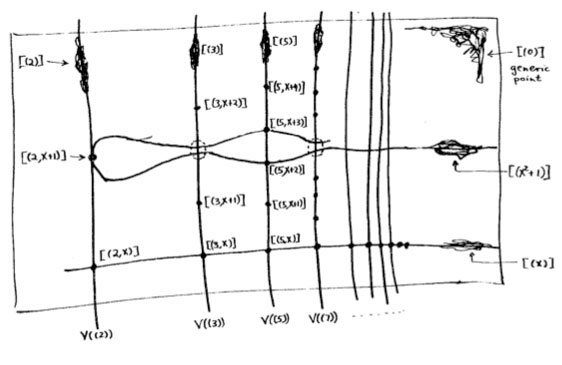
\includegraphics[width=0.9\textwidth]{media/mumforddrawing.jpg}
\end{center}
Mumford uses $[\kp]$ to denote the point $\kp$,
which we don't, so you can ignore the square brackets that appear everywhere.
The non-closed points are illustrated as balls of fuzz.

As before, there are there types of prime ideals,
but they will look somewhat more different:
\begin{itemize}
	\ii The closed points are now pairs $(p, f(x))$
	where $p$ is a prime and $f$ is an irreducible polynomial modulo $p$.
	Indeed, these are the maximal ideals:
	the quotient $\ZZ[x] / (p,f)$ becomes some finite extension of $\FF_p$.
	\ii There are now two different ``one-dimensional'' non-closed points:
	\begin{itemize}
		\ii Each rational prime gives a point $(p)$ and
		\ii Each irreducible polynomial $f$ gives a point $(f)$.
	\end{itemize}
	Indeed, note that the quotients of $\ZZ[x]$ by each are integral domains.
	\ii $\ZZ[x]$ is an integral domain,
	so as always $(0)$ is our generic point for the entire space.
\end{itemize}
There is one bit that I would do differently,
in $\VV(3)$ and $\VV(7)$, there ought to be a point $(3,x^2+1)$,
which is not drawn as a closed point in the picture,
but rather as dashed oval.
This is not right in the topological sense:
as $\km = (3, x^2+1)$ is a maximal ideal,
so it really is one closed point in the scheme.
But the reason it might be thought of as ``doubled'',
is that $\ZZ[x] / (3,x^2+1)$,
the residue field at $\km$,
is a two-dimensional $\FF_3$ vector space.

%%fakechapter 1D cut out from 2D
\section{$\Spec k[x,y]/(y-x^2)$, the parabola}
\label{sec:parabola}
By \Cref{prop:prime_quotient},
the prime ideals of $k[x,y] / (y-x^2)$
correspond to the prime ideals of $k[x,y]$ which are supersets of $(y-x^2)$,
or equivalently the points of $\Spec k[x,y]$ contained
inside the closed set $\VV(y-x^2)$.
Moreover, the subspace topology on $\VV(y-x^2)$
coincides with the topology on $\Spec k[x,y] / (y-x^2)$.

\begin{center}
\begin{asy}
	real f(real x) { return x*x; }
	draw(graph(f,-2,2,operator ..), blue, Arrows(TeXHead));
	label("$\operatorname{Spec} k[x,y]/(y-x^2)$", (0, f(0)), dir(-90), blue);
\end{asy}
\end{center}

This holds much more generally:
\begin{exercise}
	[Boring check]
	Show that if $I$ is an ideal of a ring $A$,
	then $\Spec A/I$ is homeomorphic as a topological space
	to the closed subset $\VV(I)$ of $\Spec A$.
\end{exercise}
So this is the notion of ``closed embedding'':
the parabola, which was a closed subset of $\Spec k[x,y]$,
is itself a scheme.
It will be possible to say more about this,
once we actually define the notion of a morphism.

The sheaf on this scheme only remembers the functions
on the parabola, though: the stalks are not ``inherited'', so to speak.
To see this, let's compute the stalk at the origin:
\Cref{thm:localization_commute_quotient} tells us it is
\[ k[x,y]_{(x,y)} / (y-x^2)
	\cong k[x,x^2]_{(x,x^2)}
	\cong k[x]_{(x)} \]
which is the same as the stalk
of the affine line $\Spec k[x]$ at the origin.
Intuitively, not surprising;
if one looks at any point of the parabola near the origin,
it looks essentially like a line,
as do the functions on it.

The stalk above the generic point is $\Frac(k[x,y] / (y-x^2))$:
so rational functions, with the identification that $y = x^2$.
Also unsurprising.

Finally, we note expect the parabola is actually isomorphic to $\Spec k[x]$,
since there is an isomorphism $k[x,y] / (y-x^2) \cong k[x]$
by sending $y \mapsto x^2$.
Pictorially, this looks like ``un-bending'' the hyperbola.
In general, we would hope that when two rings $A$ and $B$ are isomorphic,
then $\Spec A$ and $\Spec B$ should be ``the same''
(otherwise we would be horrified),
and we'll see later this is indeed the case.

\section{$\Spec \ZZ[i]$, the Gaussian integers (one-dimensional)}
You can play on this idea some more in the integer case.
Note that \[ \ZZ[i] \cong \ZZ[x] / (x^2+1) \]
which means this is a ``dimension-one'' closed set within $\Spec \ZZ[x]$.
In this way, we get a scheme whose elements are \emph{Gaussian primes}.

You can tell which closed points are ``bigger'' than others
by looking at the residue fields.
For example the residue field of the point $(2+i)$ is
\[ \kappa\left( (2+i) \right) = \ZZ[i] / (2+i) \cong \FF_5 \]
but the residue field of the point $(3)$ is 
\[ \kappa\left( (3) \right) \cong \ZZ[i] / (3) \cong \FF_9 \]
which is a degree two $\FF_3$-extension.

\section{Long example: $\Spec k[x,y]/(xy)$, two axes}
This is going to be our first example of a non-irreducible scheme.

\subsection{Picture}
Like before, topologically it looks like the closed set $\VV(xy)$
of $\Spec k[x,y]$.
Here is a picture:
\begin{center}
\begin{asy}
	draw( (-4,0)--(4,0), blue, Arrows);
	draw( (0,-4)--(0,4), blue, Arrows);
	dot("$(x)$", (0.3,3), dir(-45), lightred);
	dot("$(y)$", (3, 0.3), dir(135), lightred);
	draw( (0.3,3.6)--(0.3,2.4), lightred+dotted );
	draw( (2.4,0.3)--(3.6,0.3), lightred+dotted );
	dot("$(x+2)$", (-2,0), dir(-90), blue);
	dot("$(y+3)$", (0,-3), dir(0), blue);
\end{asy}
\end{center}
To make sure things are making sense:
\begin{ques}
	[Sanity check]
	Verify that $(y+3)$ is really a maximal ideal of $\Spec k[x,y] / (xy)$
	lying in $\VV(x)$.
\end{ques}

The ideal $(0)$ is longer prime,
so it is not a point of this space.
Rather, there are two non-closed points this time:
the ideals $(x)$ and $(y)$,
which can be visualized as floating around each of the two axes.
This space is reducible,
since it can be written as the union
of two proper closed sets, $\VV(x) \cup \VV(y)$.
(It is still \emph{connected}, as a topological space.)

\subsection{Throwing out the $y$-axis}
Consider the distinguished open set $U = D(x)$.
This corresponds to deleting $\VV(x)$, the $y$-axis.
Therefore we expect that $D(x)$
``is'' just $\Spec k[x]$ with the origin deleted,
and in particular that we should get $k[x, x\inv]$
for the sections.
Indeed,
\begin{align*}
	\OO_{\Spec k[x,y]/(xy)} (D(x))
	&\cong (k[x,y]/(xy))[1/x] \\
	&\cong k[x, x\inv, y] / (xy) \cong k[x, x\inv, y] / (y) \cong k[x, x\inv].
\end{align*}
where $(xy) = (y)$ follows from $x$ being a unit.
Everything as planned.

\subsection{Stalks above some points}
Let's compute the stalk above the point $\km = (x+2)$,
which we think of as the point $(-2,0)$ on the $x$-axis.
(If it makes you more comfortable, note that $\km \ni y(x+2) = 2y$
and hence $y \in \km$, so we could also write $\km = (x+2,y)$.)
The stalk is
\[ \OO_{\Spec k[x,y] / (xy), \km} = k[x,y]_{(x+2)} / (xy). \]
This might look confusing until we realize that $\frac1x$
is an element of $k[x,y]_{(x+2)}$, so $x$ is a unit;
thus $(xy)$ and $(y)$ specify the same ideal and
\[ \OO_{\Spec k[x,y] / (xy), (x+2)} \cong k[x,y]_{(x+2)} / (y)
	\cong k[x]_{(x+2)}  \]
which anyways looks just like the stalk of $(x+2)$ in $\Spec k[x]$.
That's expected.
If we have a space with two lines but we're
standing away from the origin,
then the stalk is not going to pick up the weird behavior
at that far-away point;
it only cares about what happens near $\km$,
and so it looks just like an affine line there.

The generic point $(y)$ (which floats around the $x$-axis)
will tell a similar tale:
if we look at the stalk above it,
we ought to find that it doesn't recognize the presence of the $y$-axis,
because ``nearly all'' points don't recognize it either.
To actually compute the stalk:
\[ \OO_{\Spec k[x,y] / (xy), (y)} = k[x,y]_{(y)} / (xy). \]
Again as $\frac1x$ is an element of $k[x,y]_{(y)}$,
we have $(xy) = (y)$ and thus
\[ \OO_{\Spec k[x,y] / (xy), (y)} = k[x,y]_{(y)} / (y)
	\cong k[x]_{(0)} \cong k(x). \]
which is what we expected
(it is the same as the stalk above $(0)$ in $\Spec k[x]$).

\subsection{Stalk above the origin (tricky)}
The stalk above the origin $(x,y)$ is interesting,
and has some ideas in it we won't be able to explore fully
without talking about localizations of modules.
We could of course write it as
\[ (k[x,y] / (xy))_{(x,y)}
	= k[x,y]_{(x,y)} / (xy). \]
and hence the elements should be
\[ \frac{c + (a_1 x + a_2 x^2 + \dots)
	+ (b_1 y + b_2 y^2 + \dots)}
	{c' + (a_1' x + a_2' x^2 + \dots)
	+ (b_1' y + b_2' y^2 + \dots)}
\]
where $c' \ne 0$.

You might feel unsatisfied with this characterization.
Here is some geometric intuition.
You can write the global section ring as
\[ k[x,y] / (xy) = c + (a_1 x + a_2 x^2 + \dots)
	+ (b_1 y + b_2 y^2 + \dots) \]
meaning that any global section is the sum of an $x$-polynomial
and a $y$-polynomial.
This is \emph{not} just the ring product $k[x] \times k[y]$, though:
because the constant term is shared.
So it is better thought of as pairs of polynomials in $k[x]$
and $k[y]$ which agree on the constant term.

If you like category theory, it is thus a fibered product
\[ k[x,y] / (xy) \cong k[x] \times_k k[y] \]
with morphism $k[x] \to k$ and $k[y] \to k$ by sending $x$ and $y$ to zero.
In that way, we can mostly decompose $k[x,y] / (xy)$
into its two components.

We really ought to be able to do the same as the stalk:
we wish to say that
\[ \OO_{\Spec k[x,y] / (xy), (x,y)}
	\cong k[x]_{(x)} \times_k k[y]_{(y)}. \]
English translation: a ``typical'' germ
ought to look like $\frac{3+x}{x^2+7} + \frac{4+y^3}{y^2+y+7}$,
with the $x$ and $y$ parts decoupled.
Equivalently, the stalk should consist of
pairs of $x$-germs and $y$-germs that agree at the origin.

In fact, this is true!
This might come as a surprise, but let's see why we expect this.
Suppose we take the germ
\[ \frac{1}{1-(x+y)}. \]
If we hold our breath, we could imagine expanding it as
a geometric series: $1 + (x+y) + (x+y)^2 + \dots$.
As $xy =0 $, this just becomes $1+x+x^2+x^3 + \dots + y+y^2+y^3+\dots$.
This is nonsense (as written), but nonetheless it suggests the conjecture
\[ \frac{1}{1-(x+y)} = \frac{1}{1-x} + \frac{1}{1-y} - 1 \]
which you can actually verify is true.
\begin{ques}
	Check this identity holds.
\end{ques}

Of course, this is a lot of computation just for one simple example.
Is there a way to make it general?
Yes: the key claim is that ``localization commutes with \emph{limits}''.
You can try to work out the statement now if you want, but we won't do so.
% \todo{but if we ever do sheaves of modules, then we will}

%%fakechapter 1D with holes
\section{$\Spec k[x,x\inv]$, the punctured line (or hyperbola)}
This is supposed to look like $D(x)$ of $\Spec k[x]$,
or the line with the origin deleted it.
Alternatively, we could also write
\[ k[x,x\inv] \cong k[x,y] / (xy-1) \]
so that the scheme could also be drawn as a hyperbola.

First, here's the 1D illustration.
\begin{center}
	\begin{asy}
		size(8cm);
		pair A = (-8,0); pair B = (8,0);
		draw(A--B, blue, Arrows);
		dot("$(x-3)$", (3,0), dir(-90), blue);
		dot("$(x+2)$", (-2,0), dir(-90), blue);
		dot("$(0)$", (0,1), dir(90), red);
		opendot(origin, blue+1.5);
		draw( (-6,0)..(-3,0.5)..(-1,1)--(1,1)--(3,0.5)--(6,0), dotted+red );
		label("$\operatorname{Spec} k[x,x^{-1}]$", A, dir(-90), blue);
	\end{asy}
\end{center}
We actually saw this scheme already when we took $\Spec k[x,y] / (xy)$
and looked at $D(y)$, too.
Anyways, let us compute the stalk at $(x-3)$ now; it is
\[ \OO_{\Spec k[x,x\inv], (x-3)}
	\cong k[x,x\inv]_{(x-3)}
	\cong k[x]_{(x-3)} \]
since $x\inv$ is in $k[x]_{(x-3)}$ anyways.
So again, we see that the deletion of the origin
doesn't affect the stalk at the farther away point $(x-3)$.

As mentioned, since $k[x,x\inv]$ is isomorphic to $k[x,y] / (xy-1)$,
another way to draw the visualize the same curve
would be to draw the hyperbola
(which you can imagine as flattening to give the punctured line.)
There is one generic point $(0)$ since $k[x,y]/(xy-1)$
really is an integral domain,
as well as points like $(x+2, y+1/2) = (x+2) = (y+1/2)$.
\begin{center}
	\begin{asy}
		size(7cm);
		import graph;
		graph.xaxis("$x$", -4, 4);
		graph.yaxis("$y$", -4, 4);

		real f (real x) { return 1/x; }
		draw(graph(f,-4,-0.25,operator ..), blue);
		draw(graph(f,0.25,4,operator ..), blue);
		label("$\operatorname{Spec} k[x,y] / (xy-1)$", (1,1), dir(45), blue);

		dot("$(0)$", (0.4,2), dir(225), red);
		filldraw(CR( (0.4,2), 0.3 ), opacity(0.1)+lightred, red+dotted);
		dot("$(x+2)$", (-2, f(-2)), dir(10), blue);
	\end{asy}
\end{center}

%%fakechapter 0D --- stalks above 1D
\section{$\Spec k[x]_{(x)}$, zooming in to the origin of the line}
We know already that $\OO_{\Spec A, \kp} \cong A_\kp$:
so $A_\kp$ should be the stalk at $\kp$.
In this example we will see that $\Spec A_\kp$
should be drawn sort of as this stalk, too.

We saw earlier how to draw a picture of $\Spec k[x]$.
You can also draw a picture of the stalk above the origin $(x)$,
which you might visualize as a grass or other plant
growing above $(x)$ if you like agriculture.
In that case, $\Spec k[x]_{(x)}$ might look like what happens
if you pluck out that stalk from the affine line.

\begin{center}
	\begin{asy}
		unitsize(0.7cm);
		pair A = (-5,0); pair B = (5,0);
		draw(A--B, blue, Arrows);
		draw( (-4,0)..(-2,0.5)..(-1,1)--(1,1)--(2,0.5)--(4,0), dotted+red );
		label("$\operatorname{Spec} k[x]$", A, dir(-90), blue);
		draw( (0,0)--(0,3), heavygreen);
		label("$\mathcal O_{\operatorname{Spec} k[x], (x)}$", (0,3), dir(90), heavygreen);
		dot("$(x)$", (0,0), dir(-90), blue);
		dot("$(0)$", (0.2,1), dir(45), red);
		add(shift(-9,0)*CC());
		draw("pluck", (-4.5, 1.5)--(-1.5,1.5), dir(90), black, EndArrow(TeXHead));
		// now the stalk
		draw( (0,0)--(0,3), heavygreen);
		label("$\operatorname{Spec} k[x]_{(x)}$", (0,3), dir(90), blue);
		draw( (-1,1)--(1,1), dotted+red );
		dot("$(0)$", (0.2,1), dir(45), red);
		dot("$(x)$", (0,0), dir(-90), blue);
	\end{asy}
\end{center}

Since $k[x]_{(x)}$ is a local ring
(it is the localization of a prime ideal),
this point has only one closed point: the maximal ideal $(x)$.
However, surprisingly, it has one more point:
a ``generic'' point $(0)$.
So $\Spec k[x]_{(x)}$ is a \emph{two-point space},
but it does not have the discrete topology:
$(x)$ is a closed point, but $(0)$ is not.
(This makes it a nice counter-example for exercises of various sorts.)

So, topologically what's happening is that when we zoom in to $(x)$,
the generic point $(0)$ (which was ``close to every point'') remains,
floating above the point $(x)$.

Note that the stalk above our single closed point $(x)$
is the same as it was before:
\[ \left( k[x]_{(x)} \right)_{(x)} \cong k[x]_{(x)}. \]
Indeed, in general if $R$ is a local ring with maximal ideal $\km$,
then $R_\km \cong R$:
since every element $x \notin \km$ was invertible anyways.
Thus in the picture, the stalk is drawn the same.

Similarly, the stalk above $(0)$ is the same as it was
before we plucked it out:
\[ \left( k[x]_{(x)} \right)_{(0)}
	= \Frac k[x]_{(x)} = k(x). \]
More generally:
\begin{exercise}
	Let $A$ be a ring, and $\kq \subseteq \kp$ prime ideals.
	Check that $A_\kq \cong (A_\kp)_\kq$,
	where we view $\kq$ as a prime ideal of $A_\kp$.
\end{exercise}
So when we zoom in like this, all the stalks stay the same,
even above the non-closed points.


\section{$\Spec k[x,y]_{(x,y)}$, zooming in to the origin of the plane}
The situation is more surprising if we pluck the stalk
above the origin of $\Spec k[x,y]$,
the two-dimensional plane.
The points of $\Spec k[x,y]_{(x,y)}$ are supposed to be
the prime ideals of $k[x,y]$ which are contained in $(x,y)$;
geometrically these are $(x,y)$ and the generic points passing through the origin.
For example, there will be a generic point for the parabola $(y-x^2)$
contained in $k[x,y]_{(x,y)}$,
and another one $(y-x)$ corresponding to a straight line, etc.

So we have the single closed point $(x,y)$ sitting at the bottom,
and all sorts of ``one-dimensional'' generic points floating above it:
lines, parabolas, you name it.
Finally, we have $(0)$, a generic point floating in two dimensions,
whose closure equals the entire space.
\begin{center}
	\begin{asy}
		size(6cm);
		draw( (0,0)--(0,3), heavygreen);
		label("$\operatorname{Spec} k[x,y]_{(x,y)}$", (0,3), dir(90), blue);
		draw( (-1,0.1)--(1,1.1), dotted+red );
		dot("$(3x-2y)$", (0.4,0.8), dir(-45), red);
		path p1 = (-0.5,2.5)..(0,2)..(0.5,2.5);
		draw(p1, dotted+red);
		dot("$(y-x^2)$", relpoint(p1,0.3), dir(200), red);
		path p2 = (-1,1.3)..(-0.5,1.8)..(0,1.6)..(0.5,1.4)..(1,1.9);
		draw(p2, dotted+red);
		dot("$(2y-x^3)$", relpoint(p2,0.7), dir(-45), red);
		dot("$(x,y)$", (0,0), dir(-90), blue);
		dot("$(0)$", (1.5,2.5), dir(225), red);
		filldraw(CR( (1.5,2.5), 0.5 ), opacity(0.1)+lightred, red+dotted);
	\end{asy}
\end{center}

\section{$\Spec k[x,y]_{(0)} = \Spec k(x,y)$, the stalk above the generic point}
The generic point of the plane just has stalk $\Spec k(x,y)$:
which is the spectrum of a field,
hence a single point.
The stalk remains intact as compared to when planted in $\Spec k[x,y]$;
the functions are exactly rational functions in $x$ and $y$.

% \section{$\Spec k[x,y]_{(y-x^2)}$, the stalk above the parabola}
% \section{$\Spec \ZZ_{(0)} = \Spec \QQ$}
% \section{$\Spec k[x,y]_{(0)}$, the stalk above the generic point}

%%fakechapter Problems
\section{\problemhead}
\begin{problem}
	Draw a picture of $\Spec \ZZ[1/55]$,
	describe the topology, and compute the stalk at each point.
\end{problem}

\begin{problem}
	Draw a picture of $\Spec \ZZ_{(5)}$,
	describe the topology, and compute the stalk at each point.
\end{problem}

\begin{problem}
	Let $A = (k[x,y]/(xy))[(x+y)\inv]$.
	Draw a picture of $\Spec A$.
	Show that it is not connected as a topological space.
\end{problem}

\begin{problem}
	Let $A = k[x,y]_{(y-x^2)}$.
	Draw a picture of $\Spec A$.
\end{problem}
